\chapter{Sujet de stage}
D’un point de vue technique l’équipe de lesfurets.com a décider d’abstraire les champs du formulaire ainsi que les dépendances à l’aide d'un méta-model. C'est à dire que les champs ainsi que leur dépendance épouse un format défini à un niveau d'abstraction diffèrent du code. Ils ne sont pas implémenter au moment de l'instanciation des champs mais au niveau du modèle de données sous forme d'Enum Java. L'implantation de la construction de chaque champs permet de caractériser chaque champs et de le présenter à l'utilisateur sous forme du champs voulu. De plus chaque champs connaîtrait par la suite les comportement nécessaires lors de l'évolution de ses co-dépendants.  A l’heure actuelle, l’application web est capable de transformer ce modèle de champs au format XMI pour pouvoir les exporter dans un logiciel de modélisation comme MagicDraw, Rational. Le stage débutera par un passage à d’autres format de modélisation (EMF, JSON) traiter à l'aide d'outils open-source qui permettront aux équipes de mieux visualiser le graphe des champs des formulaires ainsi que leurs dépendances. Il est prévu ensuite de superposer des analytics sur ces graphes. Il est aussi envisager de garder une trace des différences entre les versions de l’application pour visualiser les modifications et/ou les régressions en fonctions des développements. Enfin au même titre qu’un IDE classique, l’outil devrai pouvoir proposer des fonctions d’édition, de sauvegarde et de partage des données traitées.

\section{Analyse Fonctionnel}
Les utilisateurs de l’outil seront d’une part les architectes logiciel de la société, les développeurs mais aussi les business-analyste (concepteur fonctionnelle) qui pourront mieux cerner les impacts des modifications au seins du formulaire. Ils pourront aussi mieux cibler les besoin des utilisateurs du site lesfurets.com. Ainsi il faudra imaginer une interface qui pourrait s'apparenter à des wireframes qui ne sera plus l’apanage des seuls ingénieurs. On pourrai aussi proposer des interfaces différentes en fonctions des utilisateurs de l'outil et de l'utilisation qu'ils en feront.

\section{Analyse du meta-modèle}
Le meta-modèle étant déjà présent dans l'application sous un format exportable, ma première approche était d'afficher le modèle du formulaire pour trouver un moyen pertinent de l'afficher par la suite. Il m'a fallu me familiariser avec un outils de modeling MagicDraw déjà utiliser dans l'entreprise MagicDraw. Le diagramme UML présentée montre des cycles rares mais présent dans le graphe de dépendance. Le données peuvent être des "field", "group", "block", "screen" ce qui correspond respectivement à un champ du formulaire, un groupe de champs, un bloc de champs et un écran. Pour avoir une vision plus concrète de leur correspondance dans un formulaire du site vous pouvez apercevoir dans l'image numéro ci-dessous que nous somme dans l'écran "Votre Véhicule", dans le bloc "Ma demande", qu'il existe un groupe pour la recherche du véhicule, en fonction de la marque et du modèle, regroupant plusieurs champs.  De plus il existe une hiérarchie claire dans le graphe. Tous les champs sont compris au moins dans des ecrans, ils peuvent être aussi compris dans des bloc et/ou des groupes. Les group peuvent être compris dans des block mais pas l'inverse. Chaque groupe, bloc ou ecran comporte au moins champ.
\begin{center}
\vspace{0.5cm} 
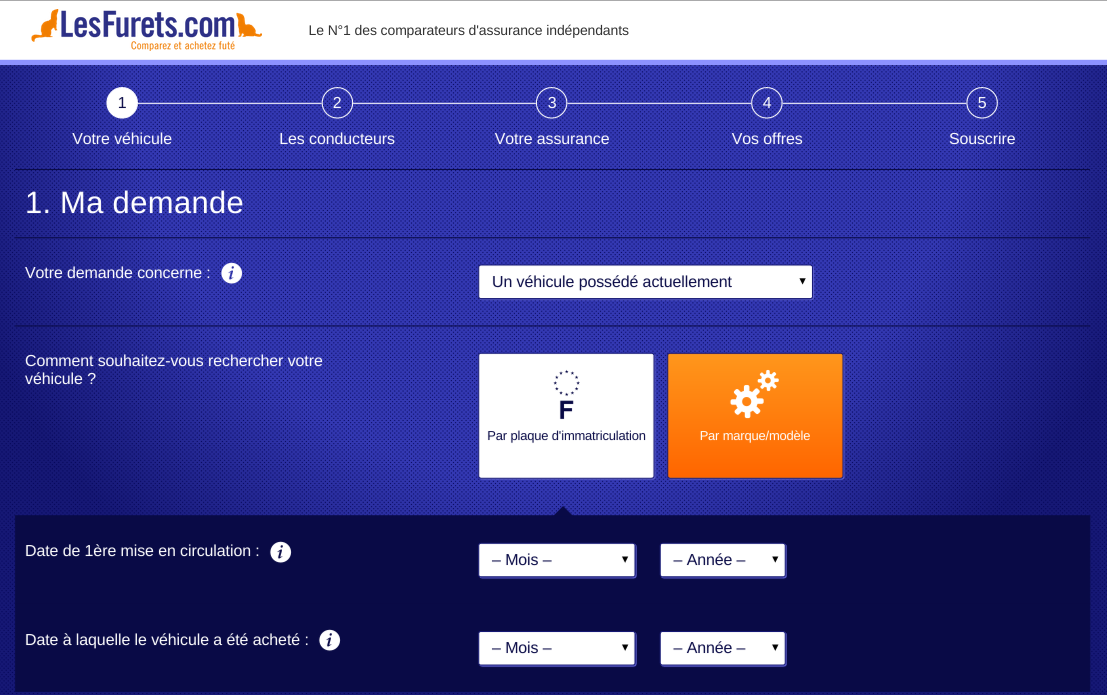
\includegraphics[height=10cm]{fields.png}
\end{center}

\section{Conception}
Dans le cadre du projet, il me faudra explorer plusieurs piste :
La première consistera à me familiariser avec un outils de modeling basé sur Eclipse : Sirius (https://eclipse.org/sirius/overview.html). Sirius est un projet Open Source de la Fondation Eclipse. Cette technologie permet de concevoir un atelier de modélisation graphique sur-mesure en s'appuyant sur les technologies Eclipse Modeling, en particulier EMF et GMF. L'atelier de modélisation créé est composé d'un ensemble d'éditeurs Eclipse (diagrammes, tables et arbres) qui permettent aux utilisateurs de créer, éditer et visualiser des modèles EMF. Le projet est une initiative française et la communauté autour du projet est très active. Je me mettrais en relations avec les créateurs du projet pour pouvoir aborder les questions que j’aurais tout au long de mon stage.
Il me faudra aussi explorer la piste de la création une application web en charge d’afficher la modélisation. Il existe de multiple librairies en JavaScript pour l’affichage des données sous la forme de graphe orienté. De plus il s'agit d'un graphe orienté faiblement cyclique qu'on pourra traitées, coté serveur avec des algorithmes implémenté en Java, Scala, Python ou JavaScript. Enfin aujourd’hui le graphe est généré sur un fichier au format XMI mais on pourrai imaginer que l’outil introspecte les objets directement dans les binaires. De plus l'approche étant donnée l'étendu de la problématique l'outils ne sera pas forcement monolithe et pourrai se repartir depuis plusieurs outils.

\section{Fonctionnalités futures}
Une fois l’outil développé et adapté aux besoin des formulaires, les équipes souhaiterait aussi modéliser d'autre donnée déjà représente par des meta-modèle au seins de l'application Java.

\subsection{Page du site}
Les pages du site, les URLs, les CSS, ainsi que la JSP utilisé sont représenté dans l'application sous forme d'Enum Java. Ainsi au même titre que pour les champs du formulaire on pourrai imaginer un outil affichant une carte des pages du site ainsi que leurs liens les unes vers les autres. Nous pourrions par la suite liée les données SEO déjà présentent et les afficher à même le graphe.

\subsection{CRM - Envoie de Mail}
L'entreprise envoie une batterie de mail aux utilisateurs une fois leur parcours fini, par exemple une fois un formulaire rempli si aucune offre nest choisi l'utilisateur peut choisir de recevoir des offres en fonction des criteres qu'il a choisi. C'est ainsi que l'application gere un nombre de regle pour un envoie de mail automatique à different moment du cycle de vie d'une fiche utilisateur.
Ce modele de mail est lui aussi abstrait grace à un modele de donnée defini dans une Enum. On pourrai comme pour les champs du formulaire imaginer de modeliser le cycle de vie d'une fiche avec le nombre d'envoie de mail, les dates et superposer les données de retour des utilisateurs en fonction des maisl envoyé.